\documentclass[a4paper]{article}

\usepackage{fullpage} % Package to use full page
\usepackage{parskip} % Package to tweak paragraph skipping
\usepackage{tikz} % Package for drawing
\usepackage{amsmath}
\usepackage{hyperref}
\documentclass{article}
\usepackage{graphicx}

\title{Summarizing, Writing and Presenting Scientific Data}
\author{Student Name:Jincheng Han \\\ 
 Student ID : 850288812}
\date{11/8/2018}

\begin{document}

\maketitle

\section{Introduction}

1.1 It was found that the \textit{Basia Indica} plant can uptake salt from water (halophyte).\\\
\\\
1.2 A set of experiemnts were conducted in order to evauate if we can use the plant to remove salt from water ("natural desalination).\\\
\\\
1.3 The experiments were conducted in an experimental wetland system and the following data was measured during the experiment. Electrical conductivity, EC (mS/cm) as a proxy for salt in the inlet and outlet of 3 wetlands (2 with plants and one without plants as a control), water and air temperature (degrees celsius), plants height.\\\
\\\
1.4 Plot the data in a useful way that will help to understand if the plants can uptake salt under the conditions in the wetlands.\\\
\\\

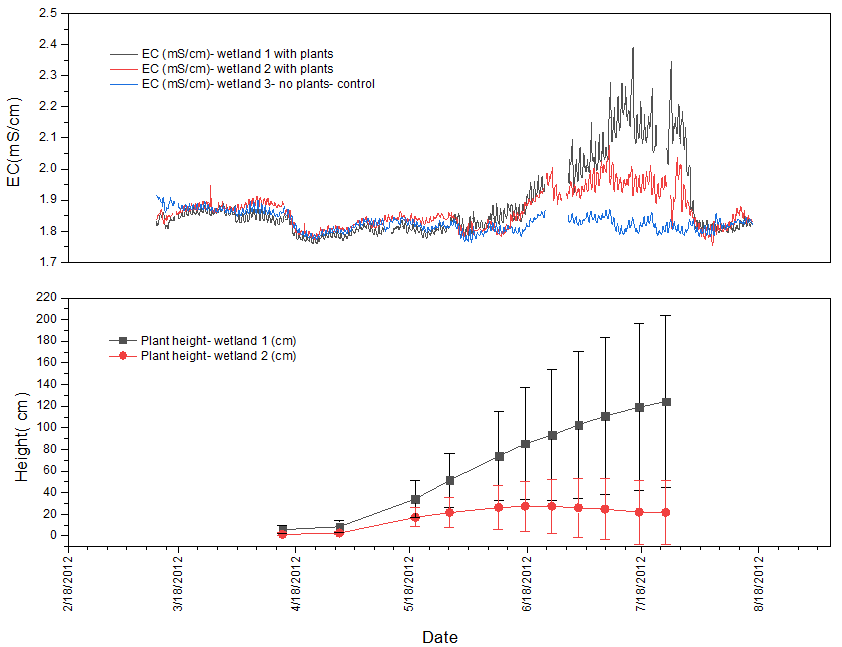
\includegraphics[width=10cm]{微信图片_20181108114817}
\centering \\\
Figure 1 \textit{Basia Indica} plant uptake salt from water. 

\end{document}